\documentclass[11pt,a4paper]{article}
\usepackage[utf8]{inputenc}
\usepackage[english]{babel}
\usepackage{amsmath}
\usepackage{amsfonts}
\usepackage{amssymb}
\usepackage{graphicx}
\usepackage{fancyhdr}
\usepackage{color}
\usepackage{listings}
\usepackage{times}

\pagestyle{fancy}
\lstset{
basicstyle=\footnotesize, 
breaklines=true
}
\begin{document}
\begin{titlepage}
\begin{center}

\includegraphics[width=0.15\textwidth]{UCL.png}
\vfill
\hrulefill
\\[1.2cm]
\textsc{\LARGE LINGI2252 Assignment 2 report}\\[1.2cm]
\hrulefill
\vfill
\begin{minipage}{0.4\textwidth}
\begin{flushleft} \large
Group 17\\
Xiao \textsc{Xu}\\ Xavier \textsc{Crochet}
\end{flushleft}
\end{minipage}
\begin{minipage}{0.4\textwidth}
\begin{flushright} \large
Kim \textsc{Mens} \\
Sergio \textsc{Castro} \\
\end{flushright}
\end{minipage}
\vfill

\includegraphics[width=0.30\textwidth]{EPL.jpg}\\
\vfill
\end{center}
\end{titlepage}


\tableofcontents
\newpage
\section{Introduction}
In the first report, we try to do a manual analysis of \textit{Glamour}. This first step gives us a global overview of \textit{Glamour} and helps us to understand how \textit{Moose} and his tools works. Because of the size of the system (about 270 classes), we use some tools in order to get some hints on where to begin. It wasn't exactly what was asked in the statement of the first report but now that we have all the tools in our hand, we can start looking more effectively for the needles in the haystack that Glamour is.\\

Moreover, we found some code duplication in the source code (but relatively few compared to the size of the framework) and the utilisation  of the \textit{Patern Obeserver} in the GLMPresentation class. We thus conclude that Glmamour was globally well-designed, despite the few code duplication.\\

The report will be divded in two parts:
\begin{enumerate}
	\item We start by analyse the code using crieria not identifiable by metrics to see
		\begin{itemize}
		\item How well the code is commented.
		\item How good the naming convetion is.
		\end{itemize}
	\item Then, we develop a set of thresolded metrics we'll use later to analyse the code.   
 \end{enumerate}
\newpage
\section{Architecture}
\subsection{Introduction}
\subsection{Overview Pyramid}
\subsection{Complexity}
\section{Comments}
Commenting code is important to improve \textbf{readability} and  the \textbf{reusability}. It make it easier for developpers to contiue a project or for student to analyse it.\\

There is so few comments in the code that we decide to not use a metric to analyse this part. In deed, there is only 768 comments! That's about 3 comments for each class.
\section{Naming Convention}

A good naming convention is also an important point in order to imrpove \textbf{readability} and \textbf{reusability} of the code. Using the \textit{Name Cloud} utility from moose, we can display the following figure, showing the most used words \textbf{for naming classes} in the framework.\\
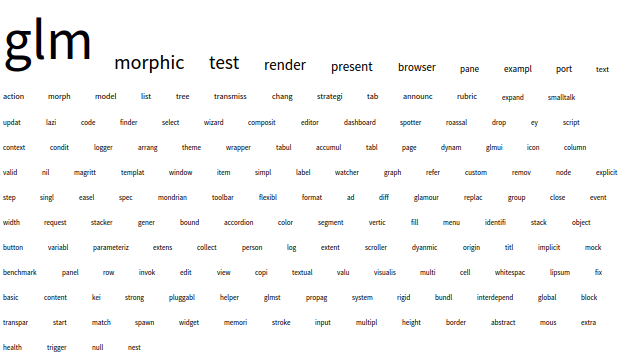
\includegraphics[width=\textwidth]{name_cloud}
\\
As we can see \textbf{GLM} is the suffix coming up the more often. Other suffix such as \textbf{test} \textbf{render} or \textbf{morphic} arise too. It seems that classes are named quite correcly in order to provide meta-information about their use.\\

We can perform the same analysis for methods or variable.Globally there is no bad smells coming up here. There is not randomly named classes variable or methods. Anyway, naming convention is quite a controversial issue, so we are not going deeper in the analysis here. 
\section{Metrics-based analysis}
\subsection{Introduction}
Before deciding when to refactor, we need first to identify where bad smells occurs inside the framework.Using \textit{Moose}'s metrics set, we start by etablishing criteria to indentify those parts.\\ 

In practice, we'll use the following query in order to retrieve the classes based on our thresholded metrics:\\

\begin{lstlisting}
((self flatCollect:[:each | each classes]) flatCollect:[:each | each methods]) select:[:each | (each ATTRIBUTE OPERATOR THRESHOLD)] 
\end{lstlisting}

If we want only to look into classes, we can do:\\
\begin{lstlisting}
(self flatCollect:[:each | each classes])  select:[:each | (each ATTRIBUTE OPERATOR THRESHOLD)]
\end{lstlisting}
%(MooseModel root allModels first) allClasses select: [:each | (each METRICNAME OPERATOR THRESHOLD)]
Avec
\begin{itemize}
\item ATTRIBUTE - The name of the attribute
\item OPERATOR - The operator for the comparaison
\item THRESHOLD - The value of the threshold
 \end{itemize}

When we wrote the first report, it appears clearly that they was some big classes in the code. We'll start by using \textit{Elephant-identifiers} attributes such as:
\begin{itemize}
\item Cohesion
\item Code Duplication
\item Larg Method and Classes
\end{itemize}

to try to explain what goes wrong inside these classes (and propose solutions).  
\subsection{Elephant-identifier attributes}
\subsubsection{Code duplication}
Having the same code structure in more than one place in the system is quite nasty. The programm will be better if we find a way to reunite them.The attributes we have to handle are \textit{NumberOfExternalDuplications} and \textit{NumberOfInternalDuplications}.\\

\textbf{Threshold} - \textit{SmallDude}, the tool used by moose to detect duplicated code have a threshold of 3 lines. We decide here to set the threshold of the two attributes to 0, and to analyse one at the time the results.\\

When querying for
\begin{itemize}
\item \textit{NumberOfInternalDuplications} we get 27 classes
\item \textit{NumberOfExternalDuplications} we get 30 classes
\end{itemize}
Let's take for example the class \textit{GLMBasicExample}.
\begin{itemize}
\item We have 3 external duplications, meaning that we have 3 block of code present in three other class of the framework. The duplication with \textit{GLMUpdateInterdepententPanesTest} is the following:
\begin{lstlisting}
browser := GLMTabulator new.
browser
	column: #one;
	column: #two;
	column: #three.
(browser transmit)
	to: #one;
	andShow:[:a] a tree display:[:x|1 to: x]].
(browser transmit)
	to: #three;
	from: #two;
\end{lstlisting}
here, we can extract a new class from \textit{GLMBasicExample} and use it inside \textit{GLMUpdateInterdepententPanesTest}.

\item We have also 6 internal duplications. The following piece of code is present two times in the class.
\begin{lstlisting}
|browser model|
	model := Dictionary new.
	model at: #some put: #(1 2 3 4).
	model at: #even put: #(2 6 8).
	model at: #odd put: #(3 7 9).
	
	browser := GLMTabulator new.
	browser column: #one.
	browser transmit to: #one; andShow: [ :a |
		a tree
			display: [model keys];  
\end{lstlisting}

We can refactor the classe by extracting the duplicated blocks as new methods, making the class more maintainable.\\

Basicly, the solution is to \textbf{extract} the duplicated block as \textbf{a new method} when  an internal one occurs, and as a \textbf{new class} when it's an external. When a external duplicated block occurs between \textbf{two parent classes}, it's more appropriate to resolve it using \textbf{inheritance}. 
\end{itemize}	
\subsubsection{Cohesion}
Cohesion metrics measure how well the methods of a class are related to each other. A cohesive class performs one function. A non-cohesive class performs two or more unrelated functions. The idea is to refactor the non-cohesive class into several smaller classes. Cohesion is thus a good thing.

The attribute to inspect here is \textit{tightClassCohesion}. It's a ratio between number of connected methods and the maximum number of possibly connected methods. Two methods are connected if they access the same attribute. 
We modify our query a little bit:
\begin{lstlisting}
(self flatCollect:[:each | each classes])  select:[:each | ((each tightClassCohesion  >= MIN) &( each tightClassCohesion < MAX))]
\end{lstlisting}

And compute the following graph, displaying the number the repartition of all the classes in term of their cohesion value.\\
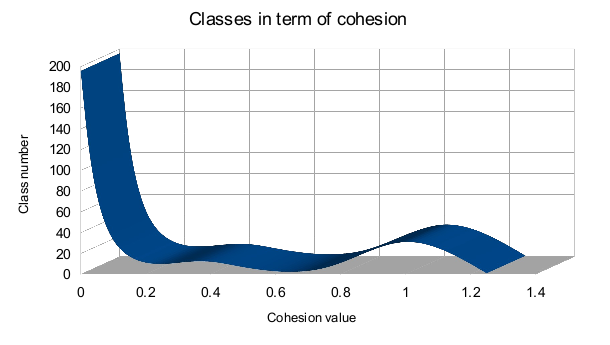
\includegraphics[width=\textwidth]{cohesion_result}

\begin{itemize}
\item We see thaht the class having the highest cohesion value (1.47) is GLMUpdateMorphicTest and has only \textbf{96 lines of codes}.\\

\item About ~200 classes have less than O.1 cohesion. 
\end{itemize}

\begin{minipage}[t]{0.4\textwidth}
When we ask moose to display the concerned classes, we see that the concerned classes are the elephant one of the framework. Furthemore, the whole \textit{GLMPresensation} Family appears on the picture (as you can see in the picture to the right):

\end{minipage}
\hfill
\begin{minipage}[t]{0.6\textwidth}
    \centering
     \vspace{-1.5ex}
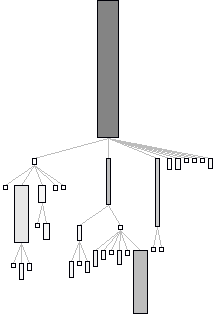
\includegraphics[width=0.6\textwidth]{GLMPresentation_family}
\end{minipage} 


Thoses classes (GLMPresentation, GLMCompositePresentation GLMListingPresentation, GLMWizard, GLMBrowser, ...)  where also identified in the first report as elephant  classes.\\
\subsubsection{Coupling}
Coupling measures the interdependance of class with other classes. Tight coupling is a bad thing. It reduces flexiblity and re-usability while increase difficulty to implements test.In order to measure coupling, we use the following metrics:
\begin{itemize}
\item fanIn : The number of classes referencing our class.
\item fanOut : The number of classes referenced by our class.
\end{itemize} 

We 
\begin{itemize}

\item compute the following metric:
$tightClassCoupling = \frac{fanOut}{fanIn}$

It measure the tightness of a class's cohesion.
\item use the following query
\begin{lstlisting}
(self flatCollect:[:each | each classes])  select:[:each | 
	(
	(each fanIn  > 0)  
	ifTrue: 
	[
	(each fanOut / each fanIn) < THRESHOLD_VALUE
	]
	ifFalse:  [ false ]
	)
]
\end{lstlisting}
\textbf{\textit{Note : to avoid having zero-fanIn result truncating result, we simply ingore them. Moreover, the 67 classes with fanIn equal to 0 correspond to all the test classes. That's why they aren't referenced in any classes.}}
\item{and compute the following graph with the collected data.}
\end{itemize}
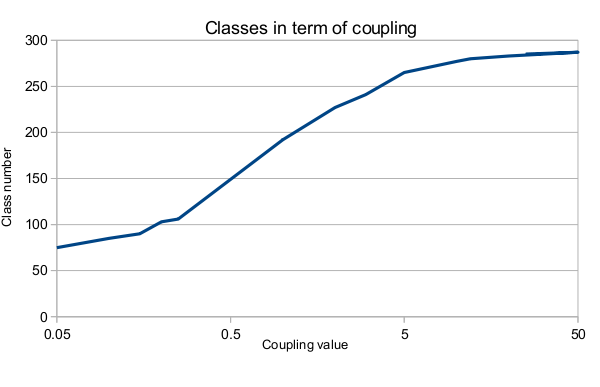
\includegraphics[width=\textwidth]{coupling_result}
\textit{Note : We use a logarithmical scale to display the x axis.}
\subsubsection{Large methods-classes}
To pursue our elephant classe analysis, we can look into these metrics:\\
\begin{tabular}{| c | c | c |}
\hline
Metric & Threshold 1 & Threshold 2\\
\hline
numberOfLinesOfCode & 25 & 30\\
\hline
numberOfStatements & 15 & 25\\
\hline
numberOfMessageSends & 10 & 20\\
\hline
\end{tabular}\\

The idea here is to look for classes having large methods doing a lot of stuff. So we look for method respecting the following rule:

\begin{quote} $ numberOfLinesOfCode > 25 \\ \vee numberOfStatements > 15 \\ \vee numberOfMessageSends > 10$\\\end{quote}

We get 196 classes. If we look at the complexity graph, these are the same classes we get on the above section. To be certain, we increase our threshod (See the second threshold of the table). We get 150 classes, among them, the one we indentify in the first report and in the previous section. 
\subsubsection{Conclusion}
If we query for classes having low cohesion, high line number of code and large methods, we get always. similar results. Even more, we reach one of our first report conclusion (We identified a large number of big classes.) We come up here the first design problem of the framework: \emph{Cohesion}. One must increase those classes's cohesion by refactoring them into smaller classes.\\

Some of the concerned classes are:\\ 

\begin{tabular}{| c | c | c | c |}
\hline 
Class Name & Lines of code & Messages sent & Cohesion\\
\hline
GLMBasicExample & 1370 & 1600 & 0.0\\
\hline
GLMPresentation & 659 & 502 & 0.076\\
\hline
GLMWhiteSpaceTheme & 778 & 524 & 0.0\\
\hline
GLMUITheme & 797 & 552 & 0.0\\
\hline
GLMCompositePresentation & 255 & 287 & 0.0051\\
\hline 
GLMWizard &  374 & 321 & 0.0029\\
\hline
GLMBrowser & 360 & 436 & 0.012\\
\hline
\end{tabular}
\subsection{Use of Object-Oriented design pattern}
\subsubsection{Introduction} 
\subsection{Accessors} 
\subsection{Long Method}
\subsection{Long Class}
\subsection{Long Parameter List}
\subsection{Conclusion}
\section{Improvements}
\section{Conclusion}
\section{Annexes}
%http://www.arisa.se/compendium/node118.html

\end{document}
